\begin{frame}{The Computational Graph}
    \framesubtitle{Why do we need them?}
    \begin{itemize}
        \item As we've seen, the output of a neural network is a deeply nested composite function.
        \item To calculate the gradient of the loss with respect to any weight, we must use the \bhighlight{chain rule} from calculus.
        \item For a network with millions of parameters, applying the chain rule manually is impossible. A \bhighlight{computational graph} is a powerful visualization tool that helps us manage this complexity and automate the process.
    \end{itemize}
\end{frame}

\begin{frame}{The Computational Graph}
    \framesubtitle{Structure}
    \begin{itemize}
        \item A computational graph represents a function as a directed graph:
        \begin{itemize}
            \item \bhighlight{Nodes (Vertices):} Represent operations (e.g., addition, multiplication) or variables.
            \item \bhighlight{Edges:} Represent the flow of data. The output of one node becomes the input to another.
        \end{itemize}
    \end{itemize}
    \begin{figure}
        \centering
        % Source: MLP & Back-prop.pdf, Page: 40
        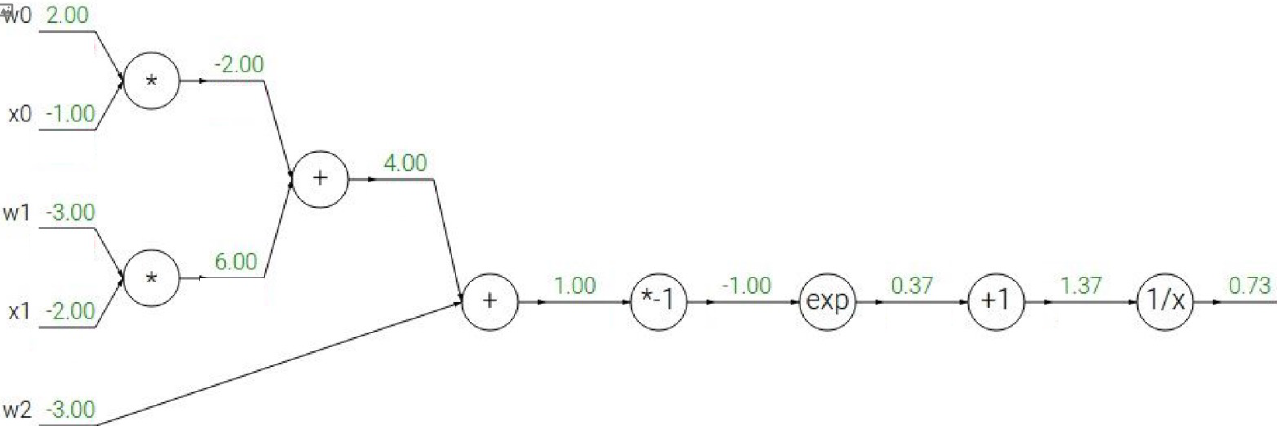
\includegraphics[width=0.9\linewidth]{images/computational_graph_sigmoid_forward.png}
        \caption{A computational graph breaking down a sigmoid neuron into its elementary operations.}
    \end{figure}
\end{frame}

\begin{frame}{The Computational Graph}
    \framesubtitle{The Forward Pass}
    \begin{itemize}
        \item The \bhighlight{forward pass} is the process of evaluating the function represented by the graph.
        \item We start from the input nodes and move forward through the graph, applying the operation at each node to the incoming values.
        \item This continues until we reach the final node, which typically represents the overall loss of the network. The path is determined by the topological sort of the graph's nodes.
    \end{itemize}
    \begin{center}
        \begin{minipage}{0.8\textwidth}
        \begin{figure}
            \centering
            % Source: MLP & Back-prop.pdf, Page: 40
            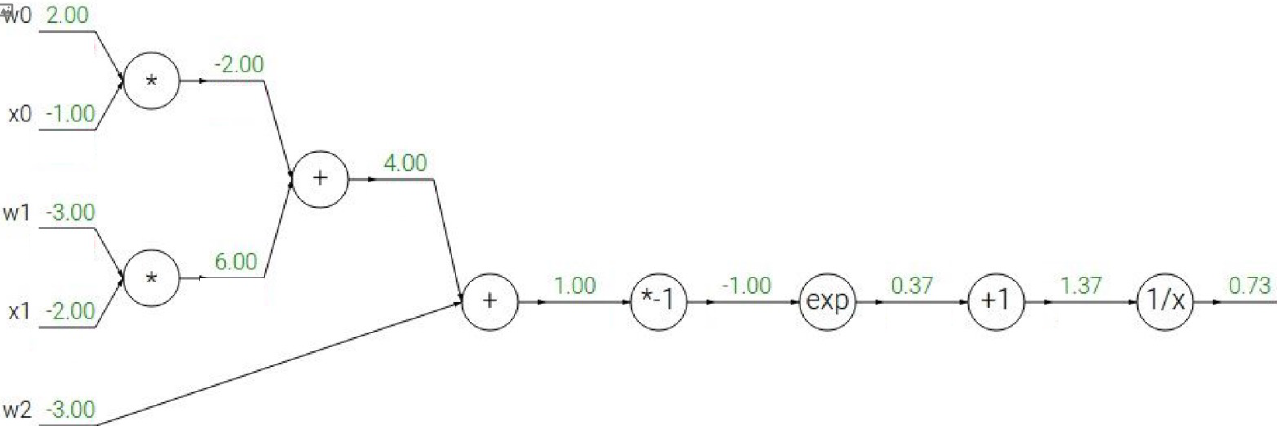
\includegraphics[width=\linewidth]{images/computational_graph_sigmoid_forward.png}
            \caption{In the forward pass, values are computed from left to right. For example, $w_0 \times x_0 = 2.00 \times -1.00 = -2.00$.}
        \end{figure}
        \end{minipage}
    \end{center}
\end{frame}

\begin{frame}{The Computational Graph}
    \framesubtitle{The Backward Pass and The Chain Rule}
    \begin{itemize}
        \item \bhighlight{Backpropagation} is the process of calculating the gradients by moving backward through the graph.
        \item At each node, we use the chain rule to compute the gradient of the final loss with respect to the node's \emph{inputs}, given the gradient with respect to its \emph{output}.
        \item We define three key terms:
        \begin{itemize}
            \item \bhighlight{Upstream Gradient ($\frac{\partial L}{\partial z}$):} The gradient coming from the nodes that follow.
            \item \bhighlight{Local Gradient ($\frac{\partial z}{\partial x}$):} The derivative of the node's operation with respect to its own inputs.
            \item \bhighlight{Downstream Gradient ($\frac{\partial L}{\partial x}$):} The gradient we want to compute and pass backward.
        \end{itemize}
        \[
            \text{Downstream Gradient} = \text{Upstream Gradient} \times \text{Local Gradient}
        \]
    \end{itemize}
\end{frame}

\begin{frame}{The Computational Graph}
    \framesubtitle{Example "Gates"}
    \begin{itemize}
        \item Different nodes (or "gates") distribute the upstream gradient in unique ways based on their local gradient:
    \end{itemize}
    \begin{figure}
        \centering
        % Source: MLP & Back-prop.pdf, Page: 38
        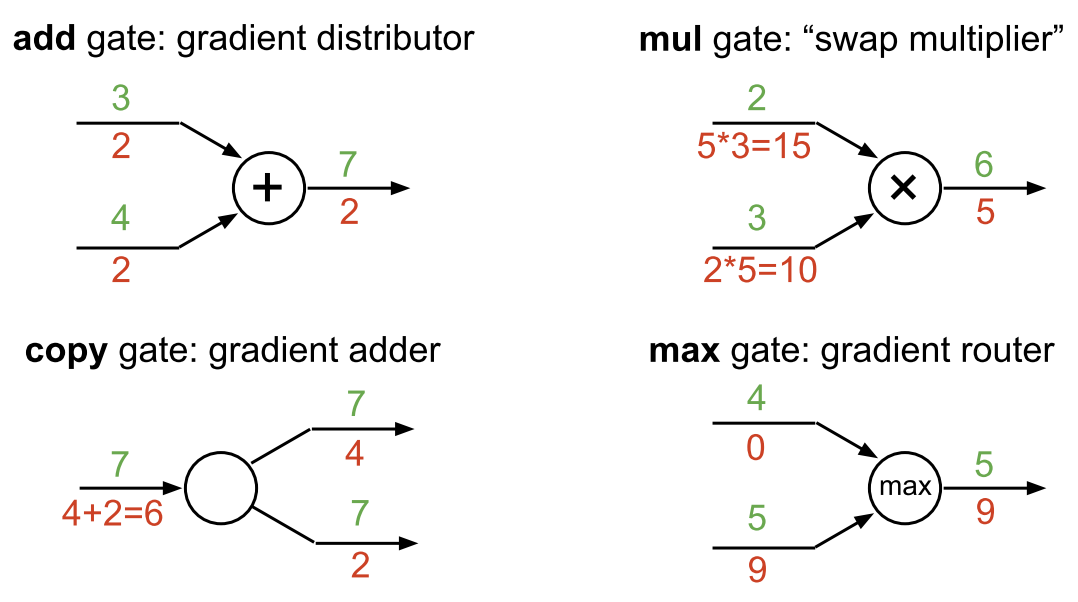
\includegraphics[width=\linewidth]{images/gradient_gates.png}
        \caption{
            \textbf{Add gate:} acts as a "gradient distributor".
            \textbf{Max gate:} acts as a "gradient router".
            \textbf{Multiply gate:} acts as a "swap multiplier".
        }
    \end{figure}
\end{frame}

\begin{frame}{The Computational Graph}
    \framesubtitle{Backpropagation Example: Step 1}
    \begin{itemize}
        \item Let's trace the backward pass for our sigmoid neuron example.
        \item We start at the very end. The gradient of the output with respect to itself is \bhighlight{1}. This is our initial upstream gradient.
    \end{itemize}
    \begin{figure}
        \centering
        % Source: MLP & Back-prop.pdf, Pages: 41-42 (combined view)
        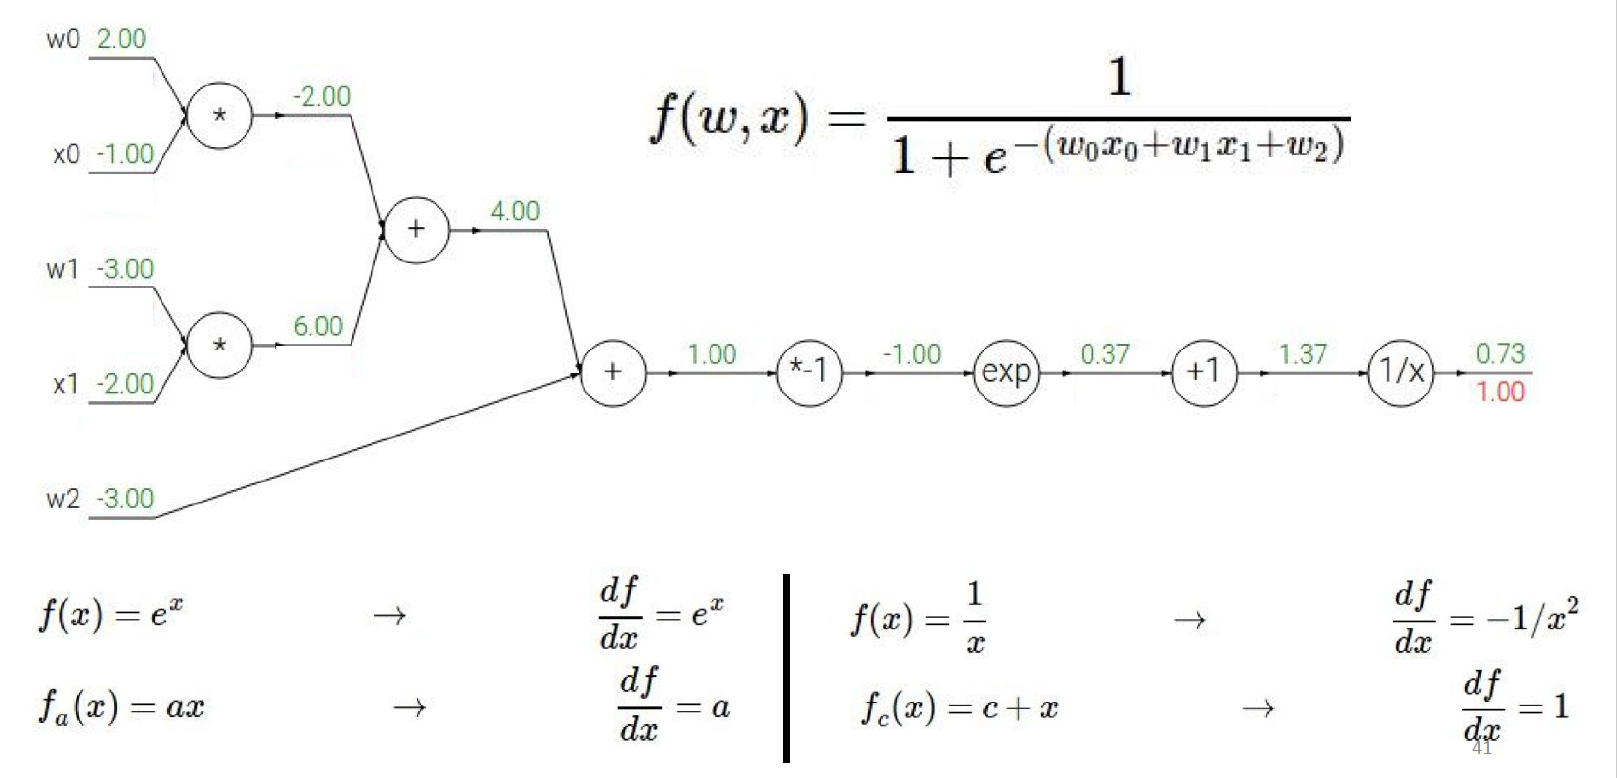
\includegraphics[width=\linewidth]{images/sigmoid_backprop_1.png}
        \caption{Starting the backward pass. The initial gradient at the output is 1.}
    \end{figure}
\end{frame}

\begin{frame}{The Computational Graph}
    \framesubtitle{Backpropagation Example: Step 2}
    \begin{itemize}
        \item The first gate is the $1/x$ gate.
        \item \textbf{Upstream Gradient}: 1.0
        \item \textbf{Local Gradient}: The derivative of $f(x) = 1/x$ is $-1/x^2$. Since the input was 1.37, the local gradient is $-1/(1.37^2) \approx -0.53$.
        \item \textbf{Downstream Gradient}: $1.0 \times -0.53 = -0.53$.
    \end{itemize}
    \begin{figure}
        \centering
        % Source: MLP & Back-prop.pdf, Page: 43
        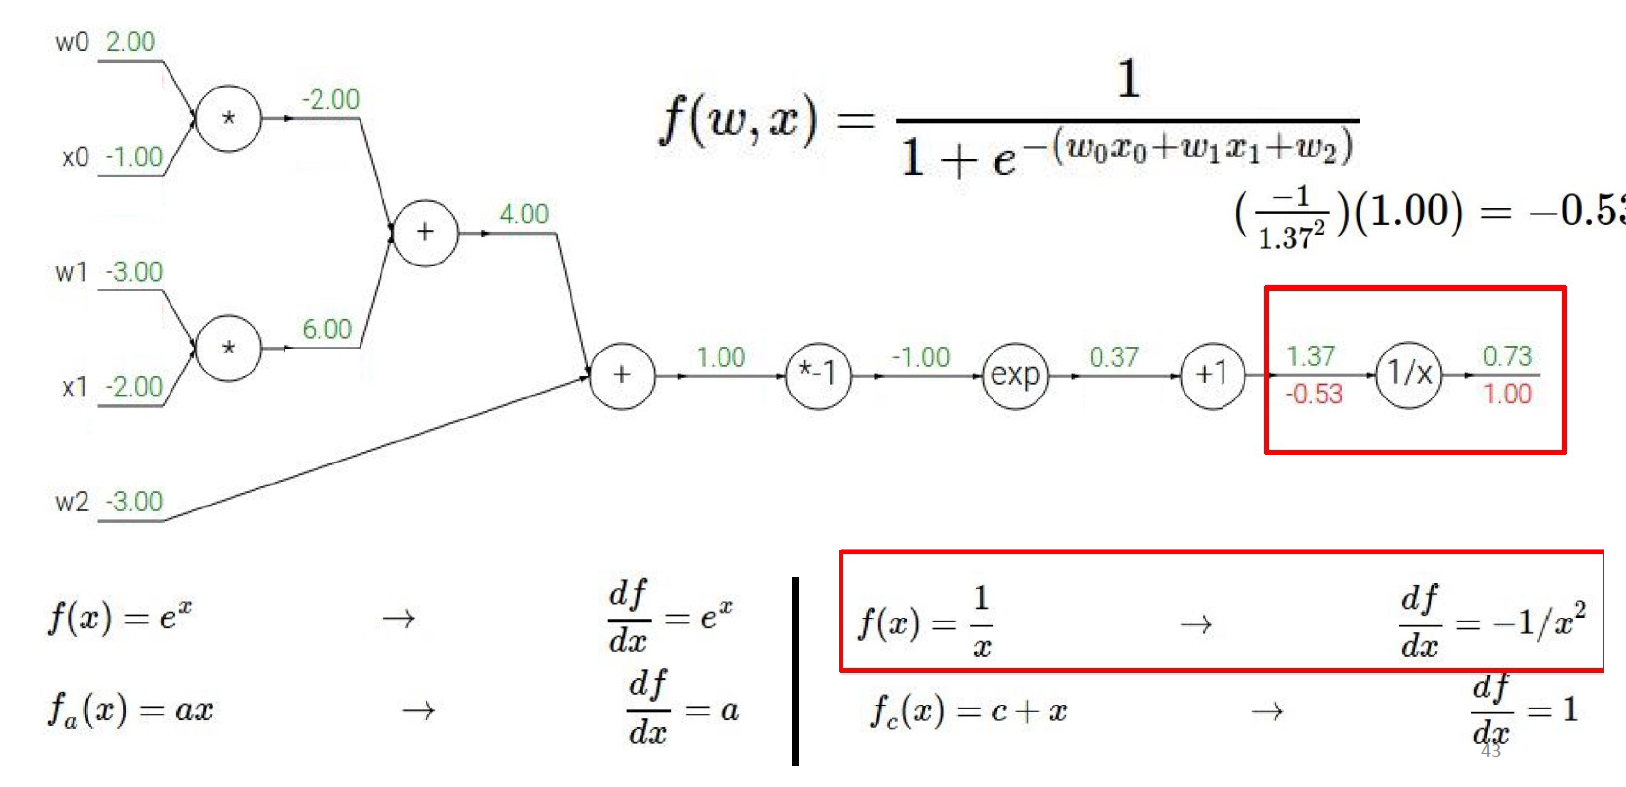
\includegraphics[width=\linewidth]{images/sigmoid_backprop_2.png}
    \end{figure}
\end{frame}

\begin{frame}{The Computational Graph}
    \framesubtitle{Backpropagation Example: Step 3}
    \begin{itemize}
        \item The next gate is the `+1` gate.
        \item \textbf{Upstream Gradient}: -0.53
        \item \textbf{Local Gradient}: The derivative of $f(x) = x+c$ is 1.
        \item \textbf{Downstream Gradient}: $-0.53 \times 1 = -0.53$.
    \end{itemize}
    \begin{figure}
        \centering
        % Source: MLP & Back-prop.pdf, Page: 45
        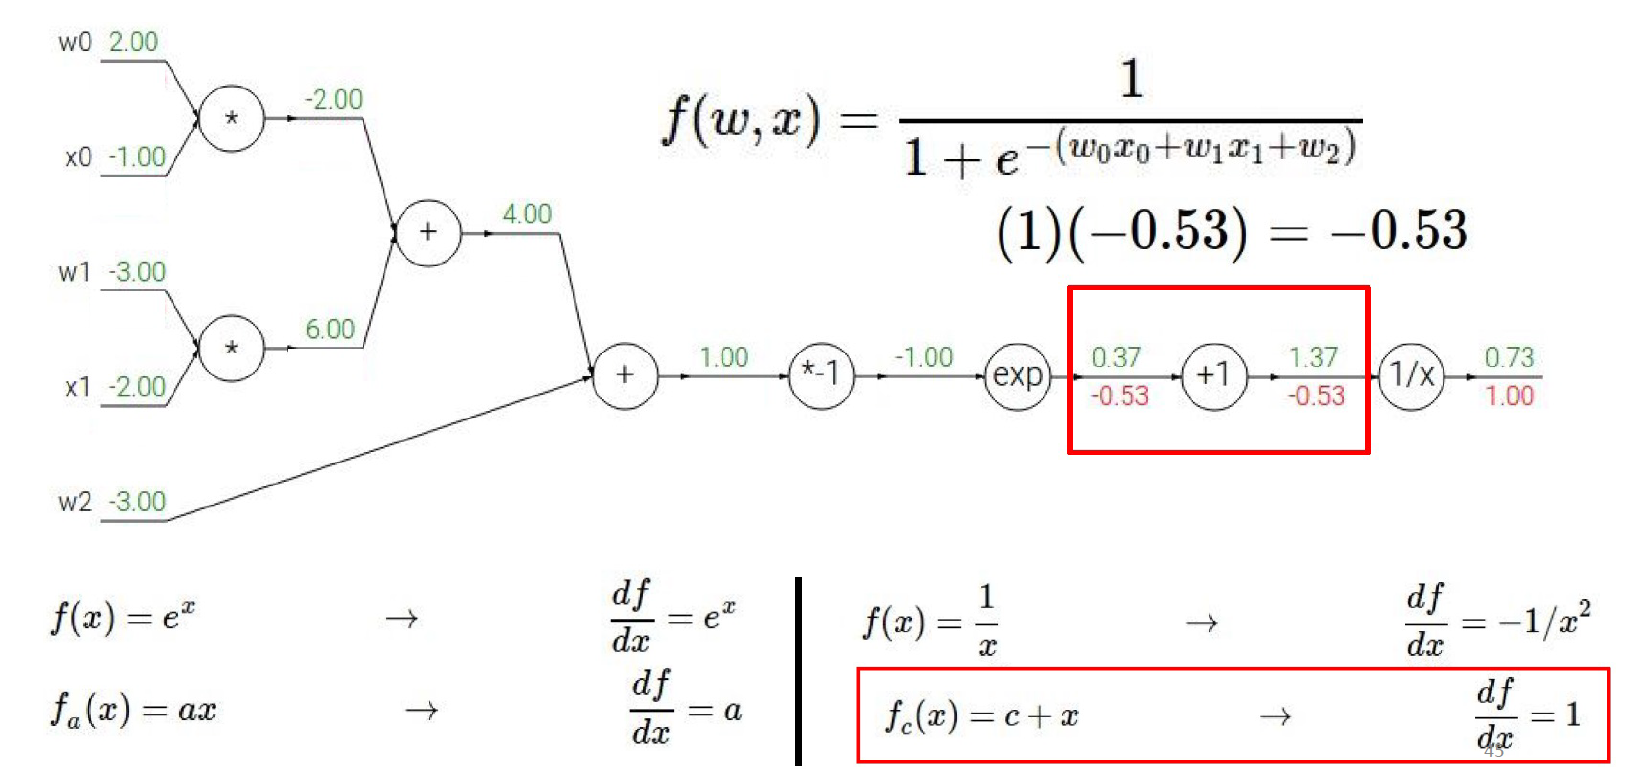
\includegraphics[width=\linewidth]{images/sigmoid_backprop_3.png}
    \end{figure}
\end{frame}

\begin{frame}{The Computational Graph}
    \framesubtitle{Backpropagation Example: Step 4}
    \begin{itemize}
        \item Next is the `exp` gate.
        \item \textbf{Upstream Gradient}: -0.53
        \item \textbf{Local Gradient}: The derivative of $f(x) = e^x$ is $e^x$. Since the input was -1.0, the local gradient is $e^{-1} \approx 0.37$.
        \item \textbf{Downstream Gradient}: $-0.53 \times 0.37 \approx -0.20$.
    \end{itemize}
    \begin{figure}
        \centering
        % Source: MLP & Back-prop.pdf, Page: 48
        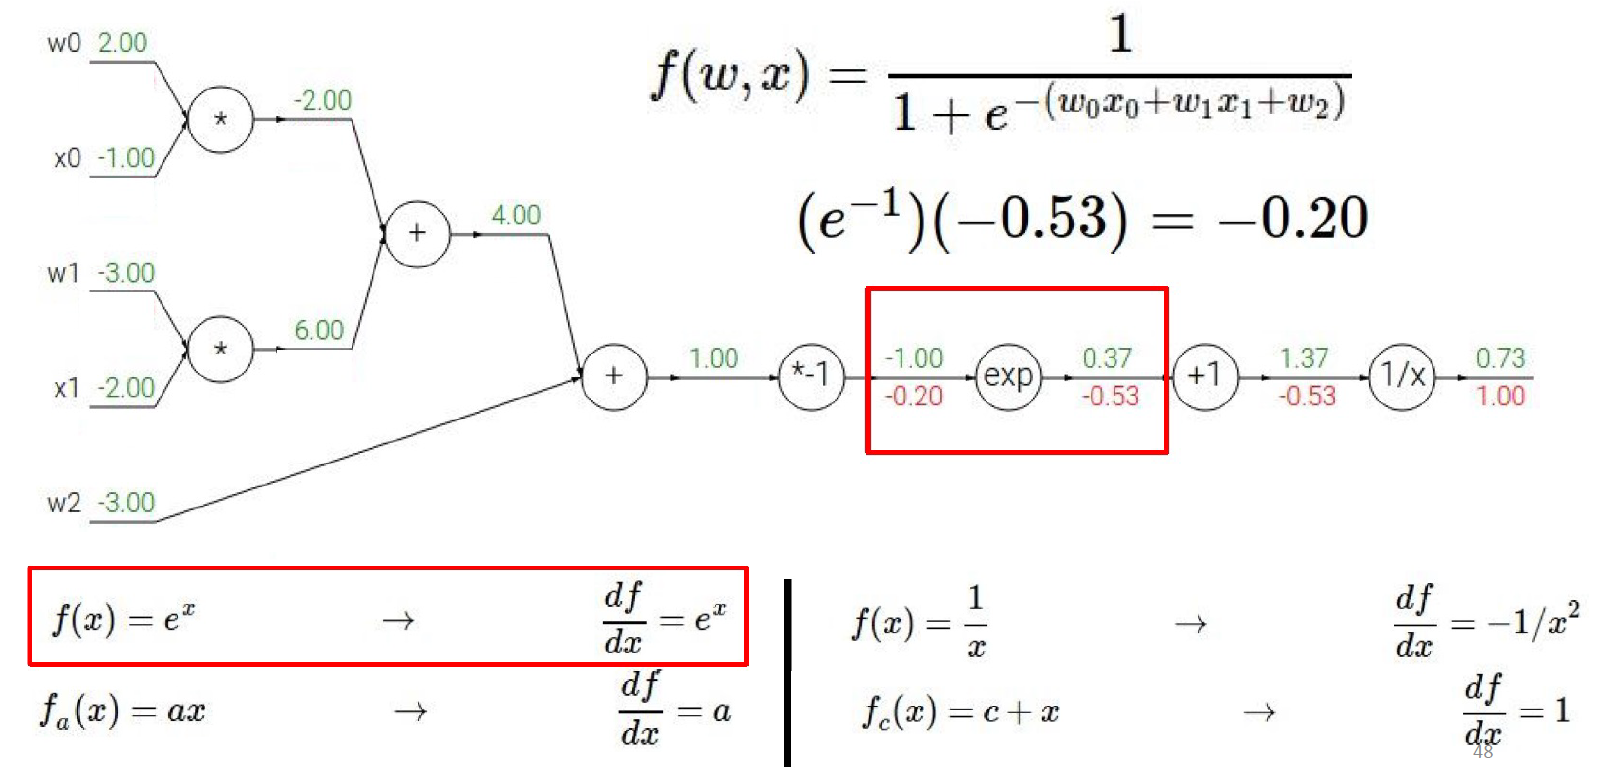
\includegraphics[width=\linewidth]{images/sigmoid_backprop_4.png}
    \end{figure}
\end{frame}

\begin{frame}{The Computational Graph}
    \framesubtitle{Backpropagation Example: Final Steps}
    \begin{itemize}
        \item The gradient is propagated backward through the remaining gates (`*-1`, `+`, `*`).
        \item For example, at the top-most `*` gate (for $w_0, x_0$):
        \begin{itemize}
            \item \textbf{Upstream Gradient}: 0.20 (from the final `+` gate).
            \item \textbf{Local Gradient} for $w_0$: The other input, $x_0 = -1.00$.
            \item \textbf{Downstream Gradient} for $w_0$: $0.20 \times -1.00 = -0.20$.
        \end{itemize}
        \item This process is repeated until we have the gradient for every weight and input.
    \end{itemize}
    \begin{figure}
        \centering
        % Source: MLP & Back-prop.pdf, Page: 53
        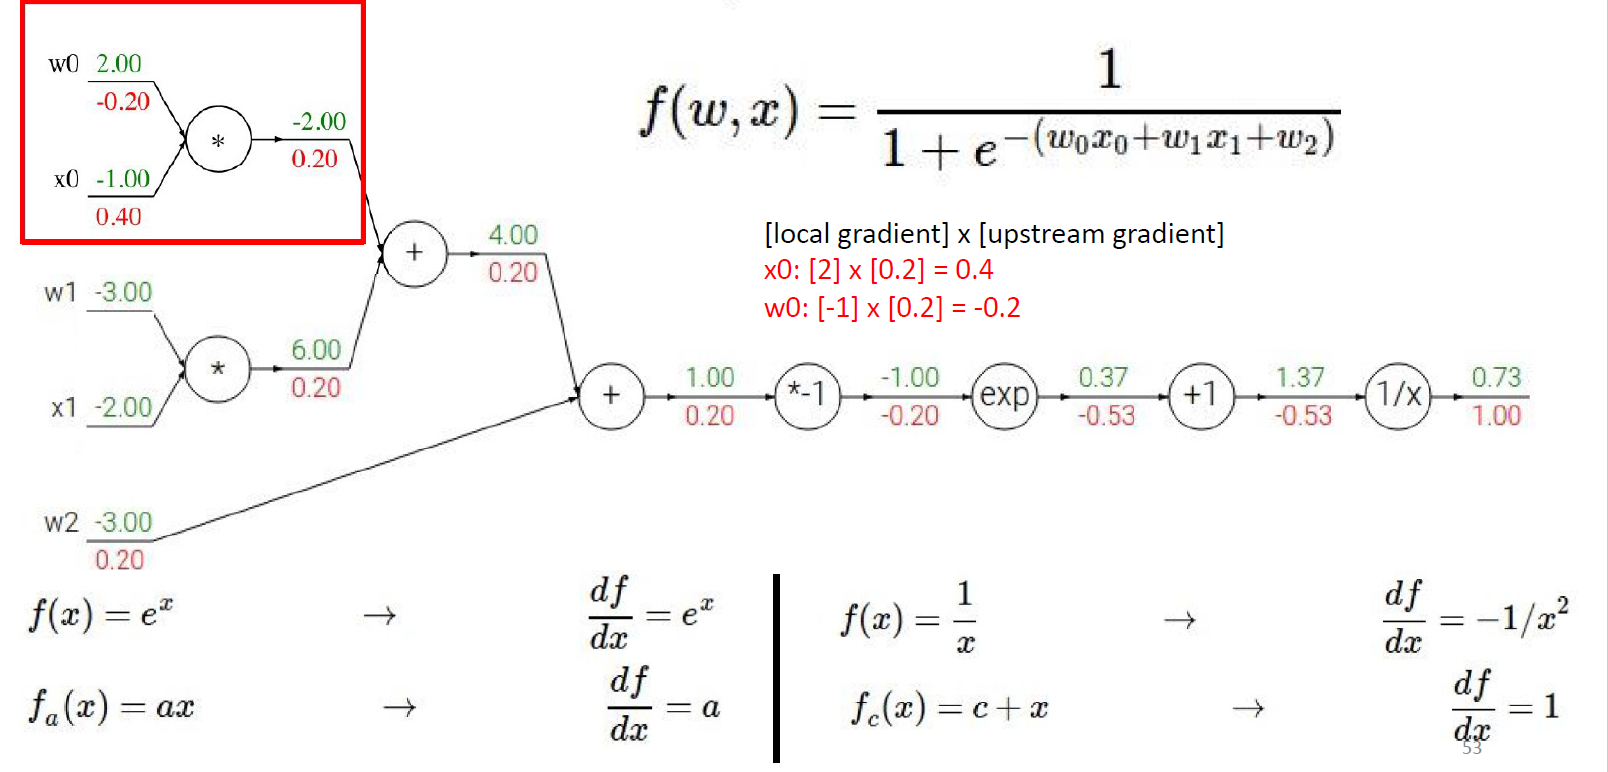
\includegraphics[width=\linewidth]{images/sigmoid_backprop_final.png}
        \caption{The final computed gradients for each weight and input.}
    \end{figure}
\end{frame}